\section{WURC Array 4x4}
\label{sec_wurc_4x4}

	Building upon the single-radio \ac{WURC} module developed in Section~\ref{sec_wurc_module}, we constructed a 4x4 \ac{MU-MIMO} testbed using the WARPv3 platform augmented with the \ac{WURC} UHF-band \ac{SDR} modules (Figure~\ref{fig_wurc_4x4_testbed}).
	
	
% WURC 4x4 Testbed system diagram
\begin{figure}[p] 
\centering
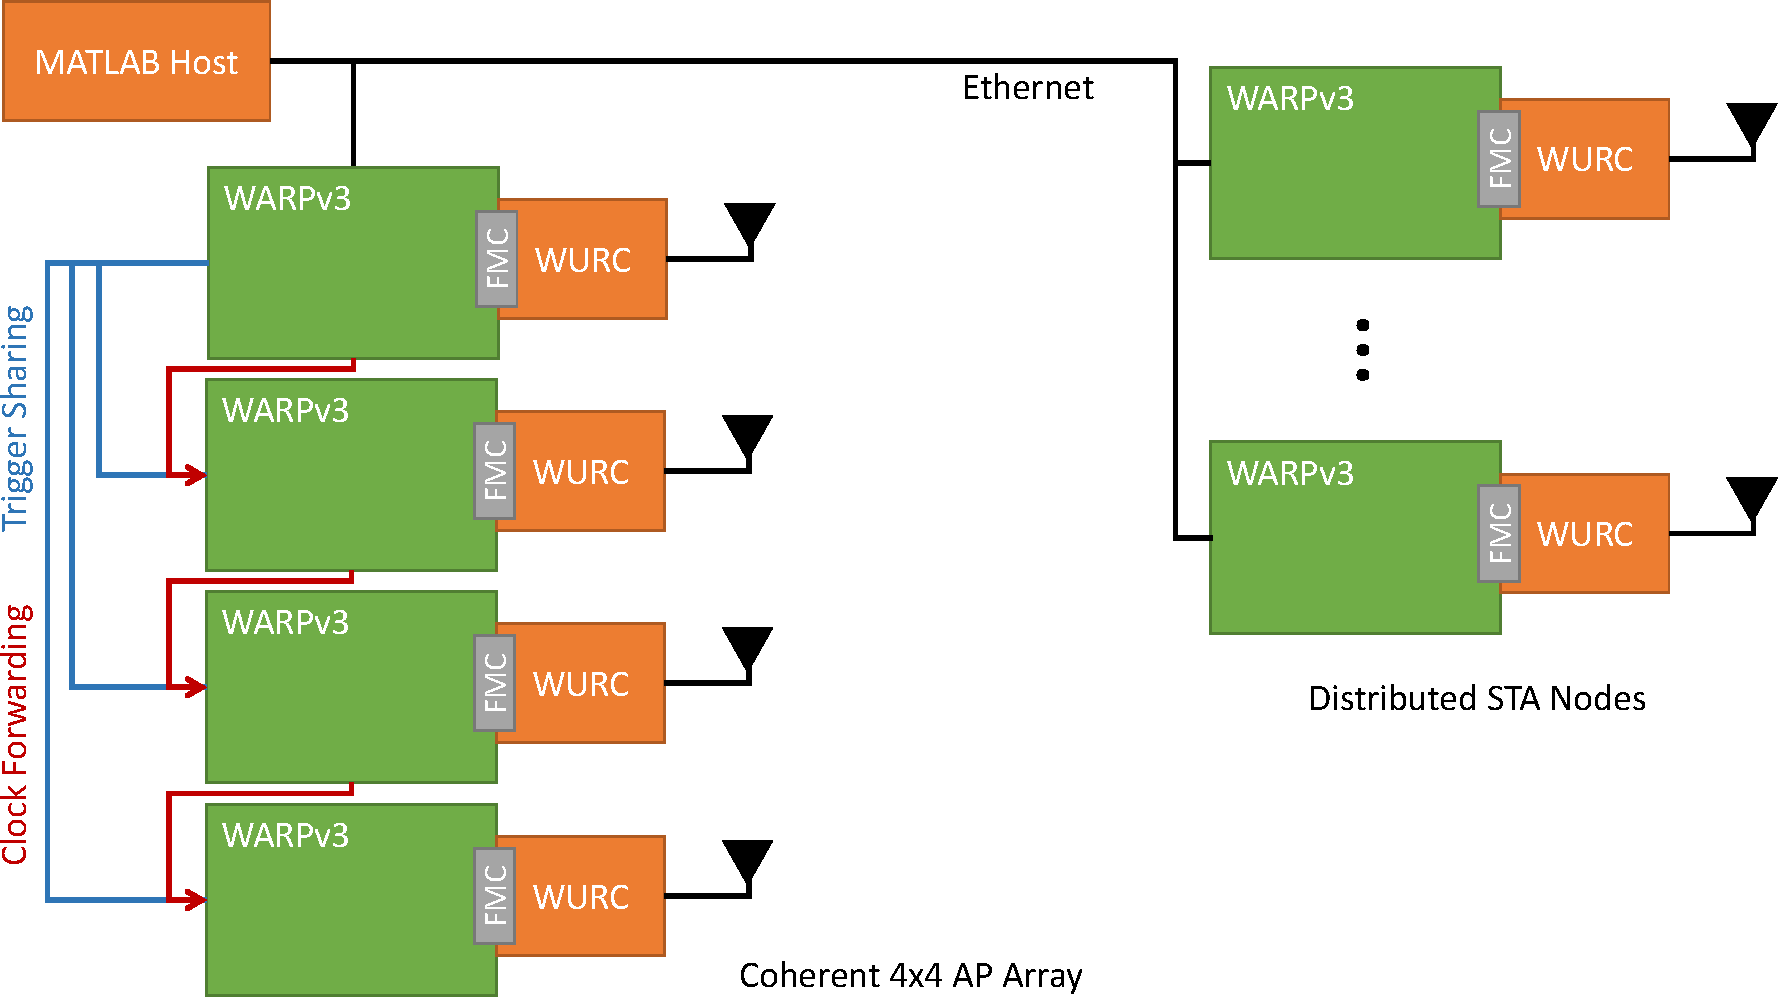
\includegraphics[width=0.9\linewidth]{./figs/wurc/wurc_warplab_sys_diagram}
\caption{System diagram of the $4\times4$ WARPLab-WURC \ac{AP} and \acp{STA}.}
\label{fig_wurc_4x4_sys_diagram}
\end{figure}

% WURC 4x4 Testbed photos
\begin{figure}[p]
\centering        
   	\subfigure[\ac{WURC} Array Internals.]{
		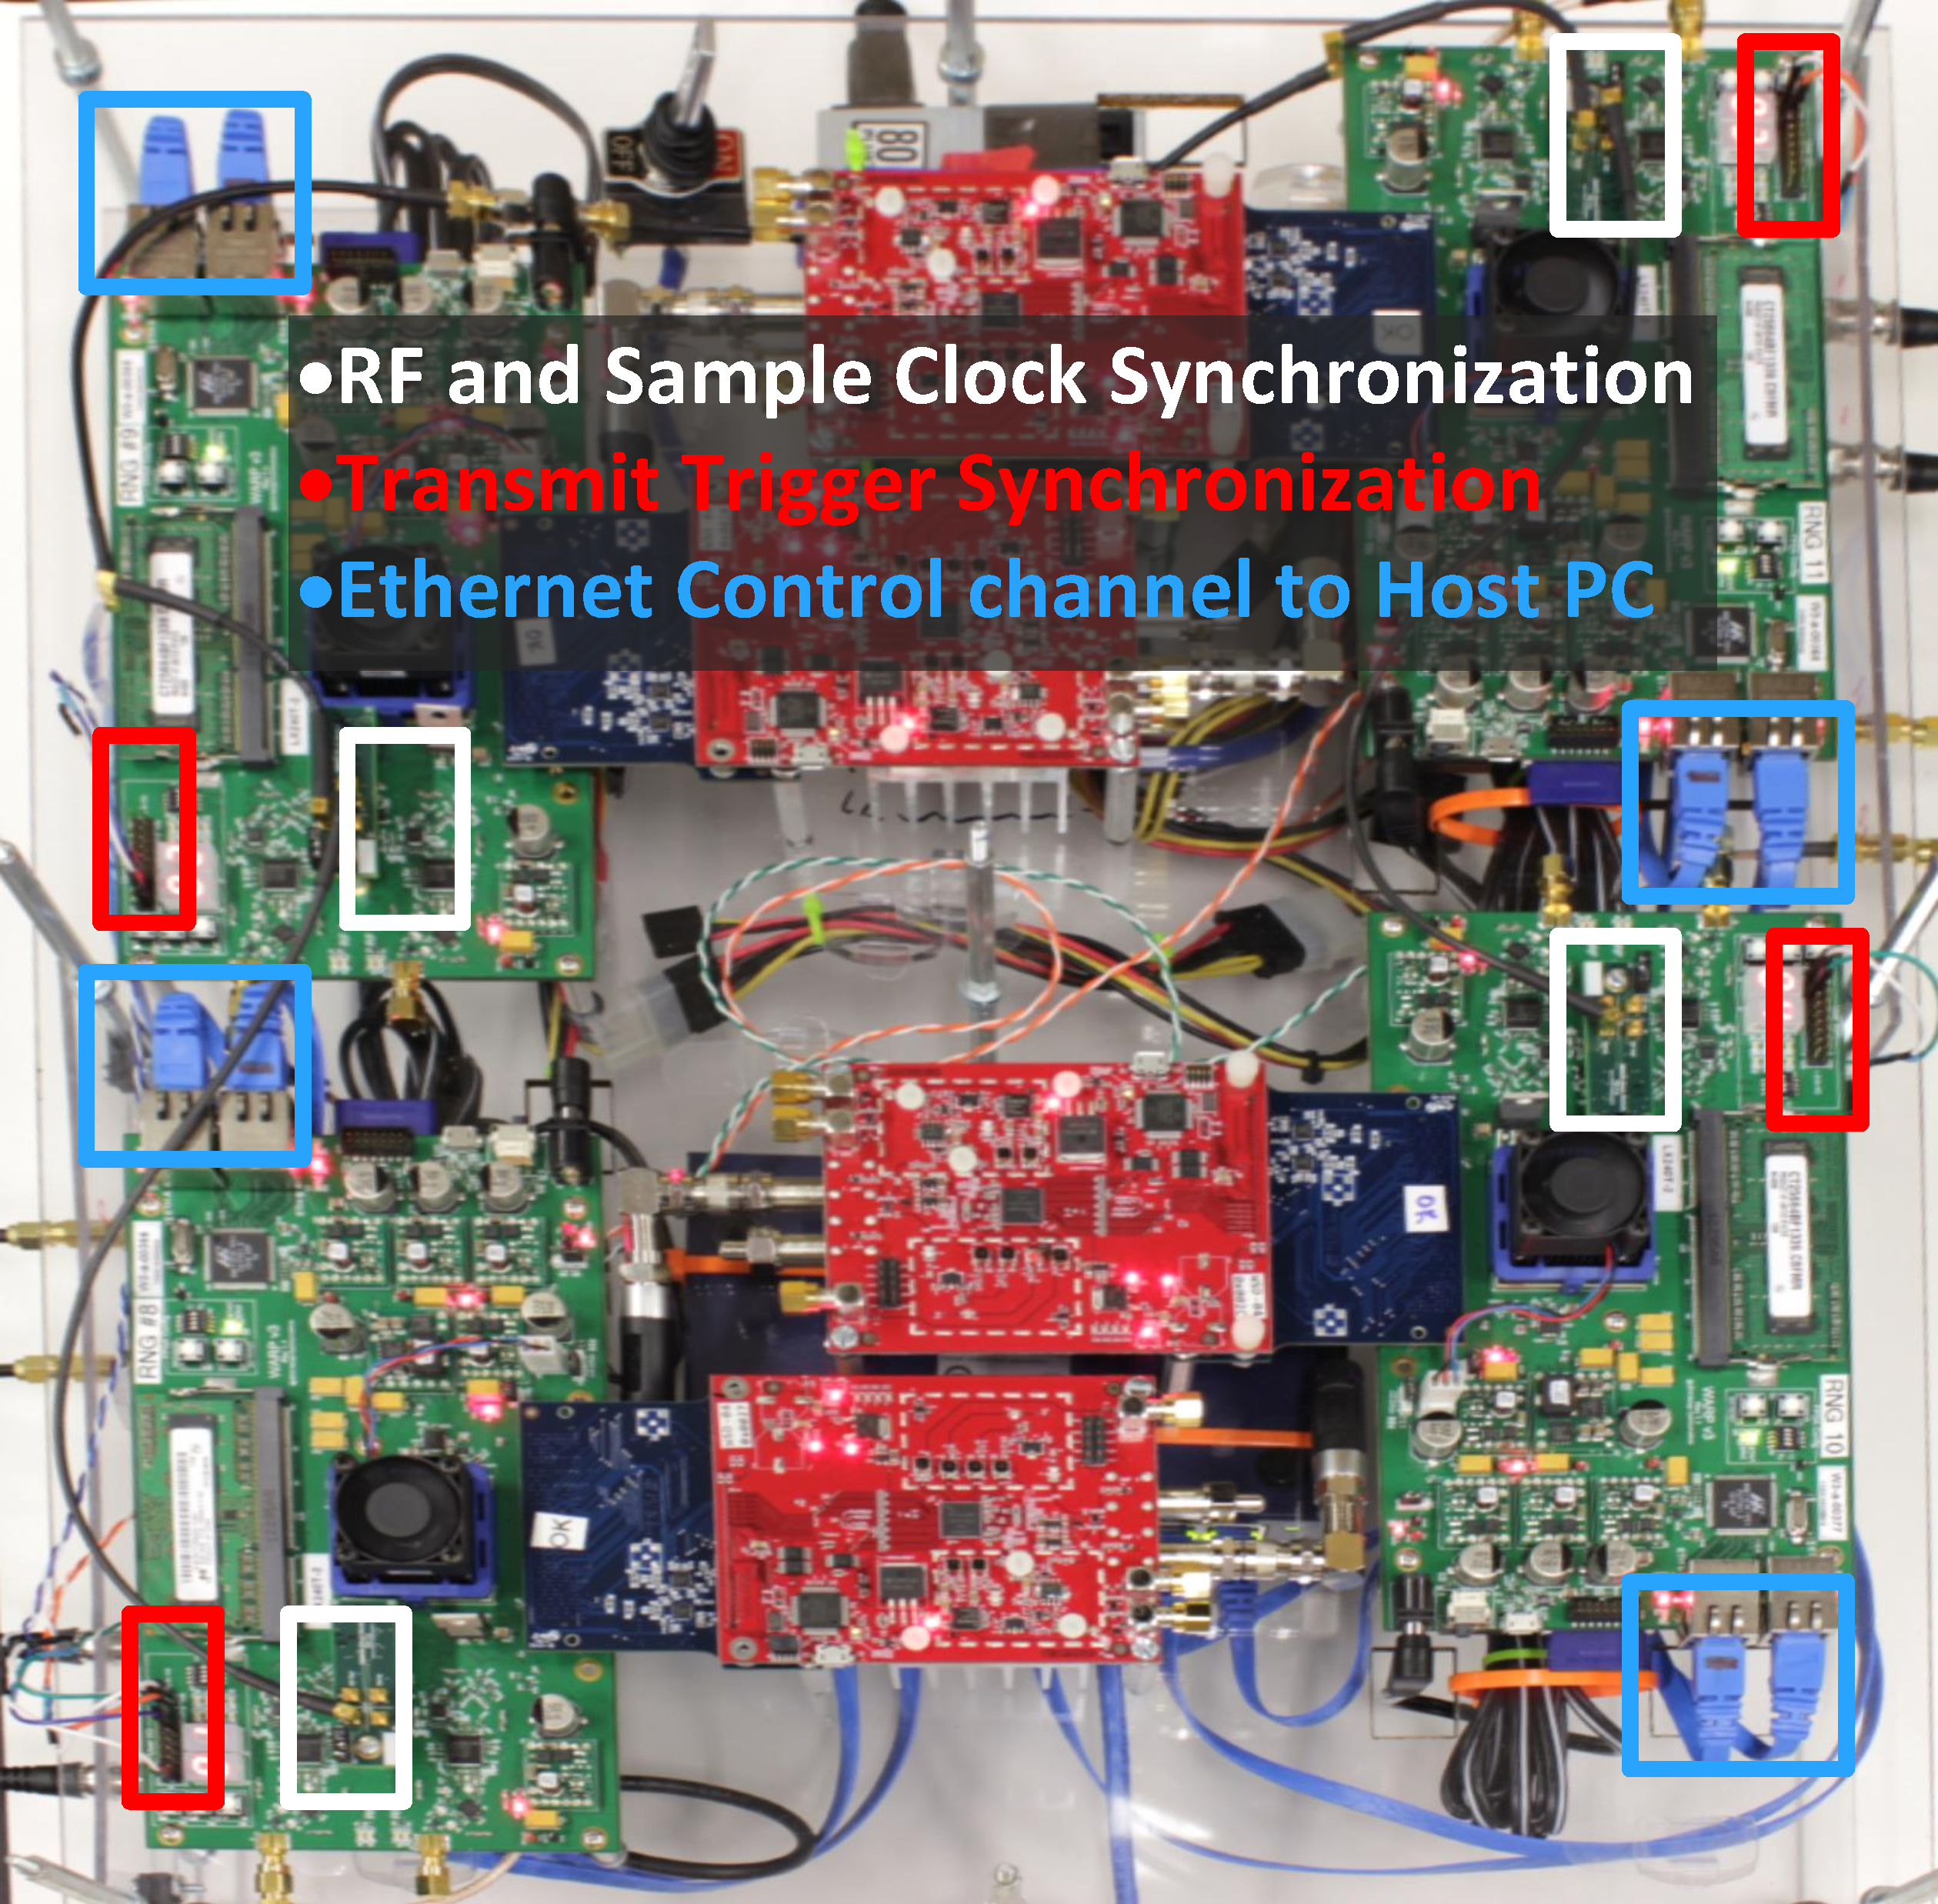
\includegraphics[width=0.45\linewidth]{figs/wurc/wurc_array_2}   \label{fig_wurcarray}
        	}
	\subfigure[\ac{WURC} Array Antennas.]{
		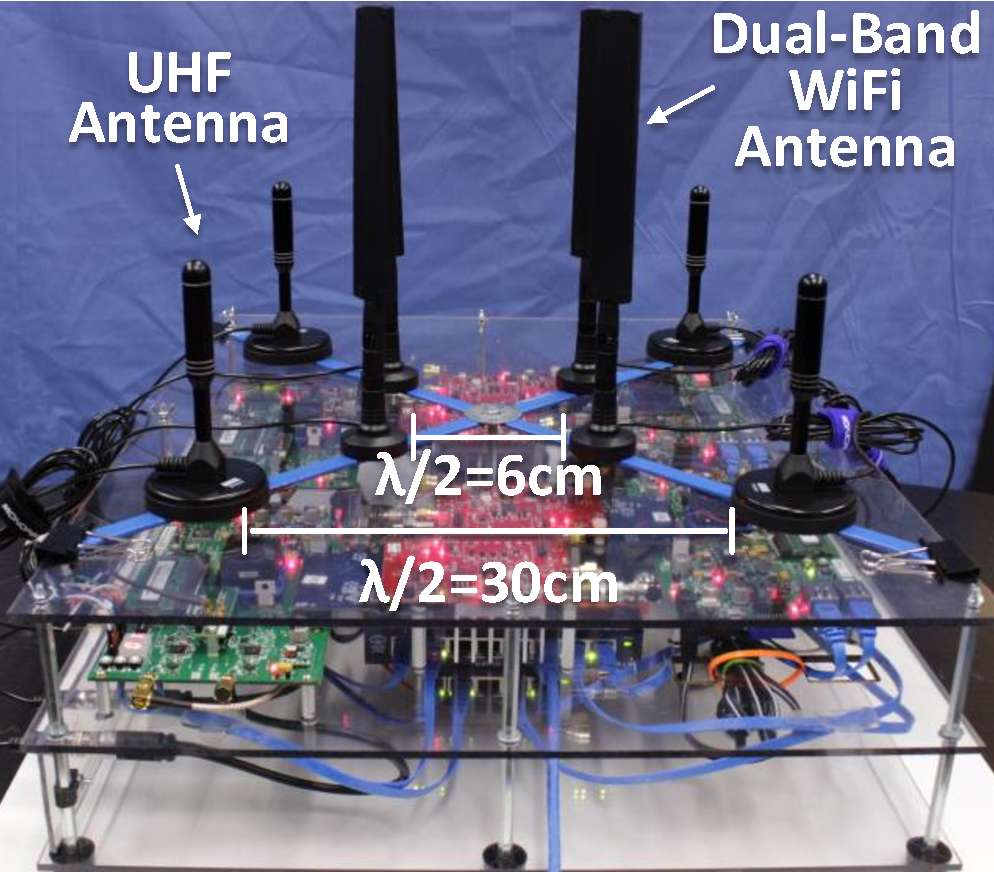
\includegraphics[width=0.45\linewidth]{figs/wurc/wurc_array_3}   \label{fig_wurcarrayTop}
        	}
\caption{Photo of the implemented $4\times4$ WARPLab-WURC \ac{AP} for UHF-band operation.
\label{fig_wurc_4x4_testbed}}
\end{figure}
	
	Utilizing the \ac{ISM}-band 2.4~GHz and 5.8~GHz radios on the WARPv3 platform as well as the 470-698~MHz UHF radios on the \ac{WURC}, we were able to build an \ac{SDR} \ac{MU-MIMO} platform with the largest operational tuning range available at the time.
	A key design consideration was to enable the use of a wide range of frequencies using the same \ac{MAC} and \ac{PHY}, allowing side-by-side comparison of performance in various RF environments.
		Each radio on each node can respectively transmit the similar 802.11af, 802.11g, and 802.11b-like \ac{OFDM} sounding and payload waveforms, controlling the \ac{PHY} implementation as an experimental variable that remains constant.
	
	The designed platform and experimental topology with an arbitrary number of distributed \ac{STA} nodes is shown in Figure~\ref{fig_wurc_4x4_sys_diagram}.


%\begin{figure}[b!]
		%\centering  
	%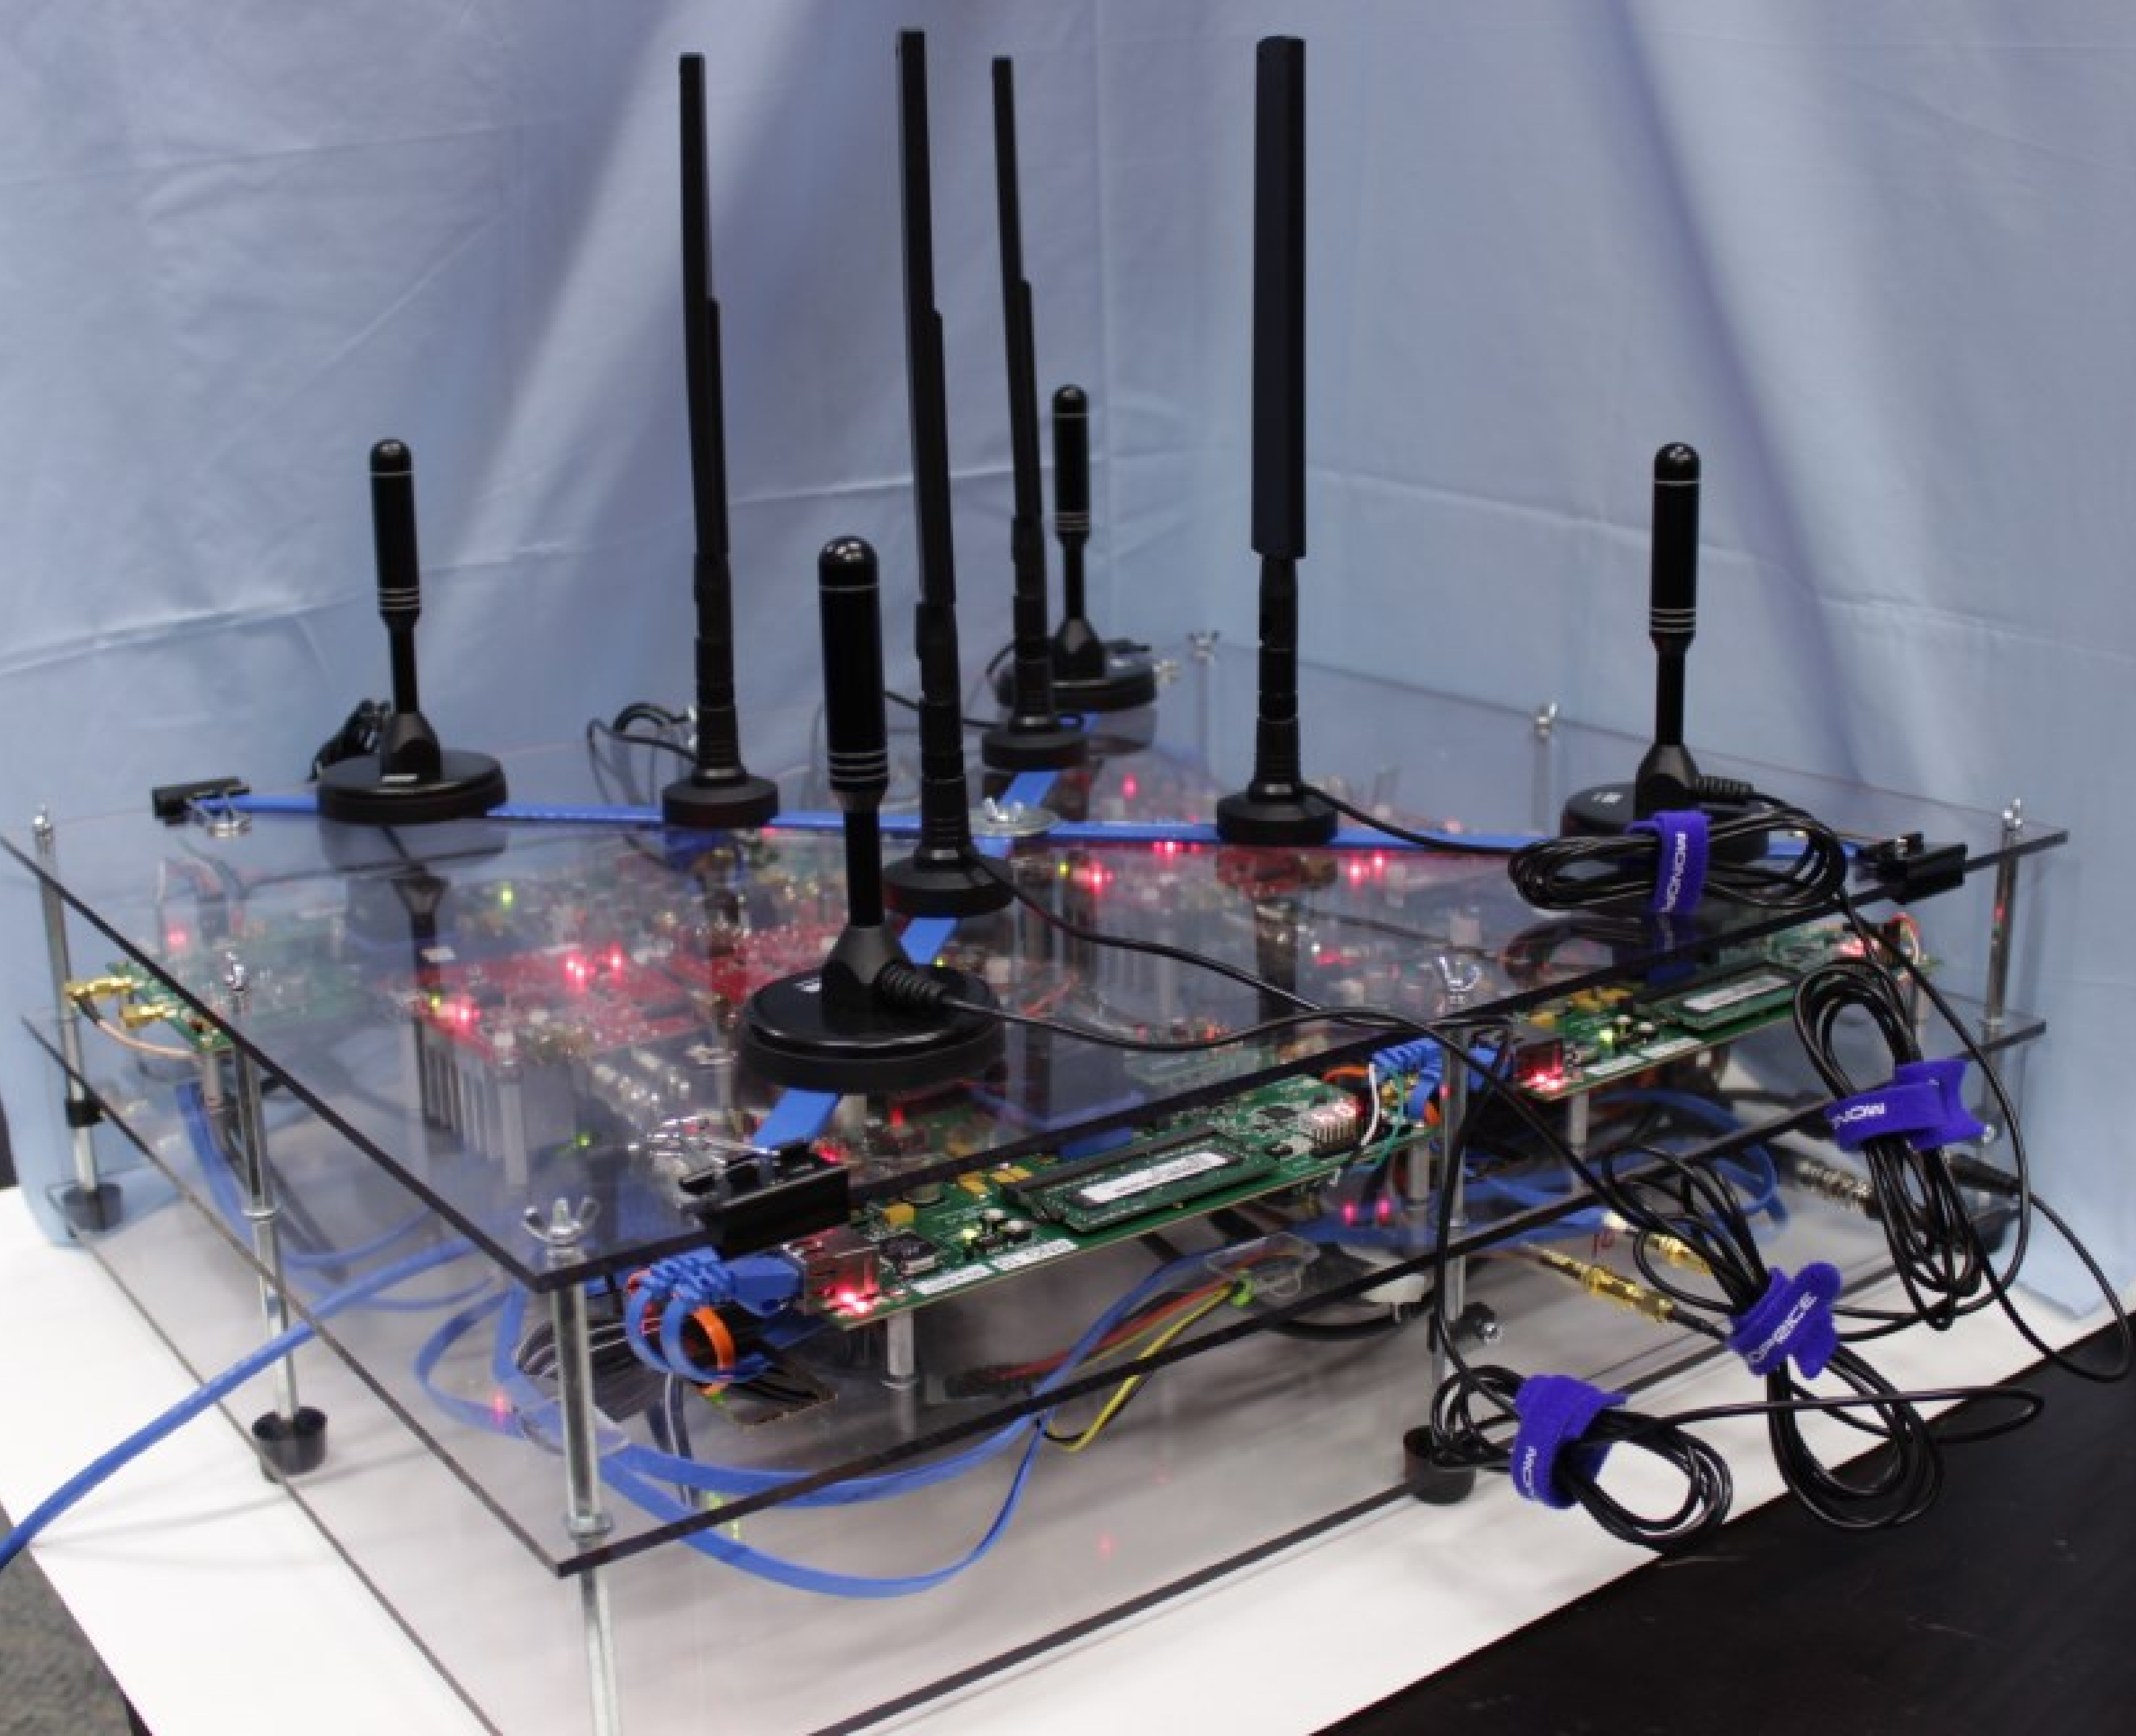
\includegraphics[width=4.5in]{figs/wurc/wurc_array_1} 
   	 %\caption{The \ac{WURC}-enabled MU-MIMO array.\label{fig:wurc_array_iso}}
%\end{figure}

%In order to evaluate \ac{MU-MIMO} transmissions at various carrier frequencies and node topologies, we integrate \ac{WURC} and four WARPv3 modules into a coherent 4-radio array.

\subsubsection{Timing and Clock Synchronization}
	The \ac{MU-MIMO} \ac{WURC} array combines four WARPv3 boards and 4 \ac{WURC} daughtercards into a single prototype base station providing combined sample and RF-reference clock synchronization, power, and structural support.
	Synchronization of reference clocks for ADC sampling and RF frequency synthesizers is required for coherent beamforming and is accomplished by forwarding a daisy-chained reference clock from one master WARPv3 baseband board to the others in the array as shown by the red clocking lines in Figure~\ref{fig_wurc_4x4_sys_diagram}
	All radios derive their sampling and RF reference clocks from this forwarded clock and thus remain phase-synchronized for transmit and receive beamforming.
	In addition, we ensure symbol timing synchronization by designating a master node that transmits a \ac{GPIO} pulse to any number of slave WARPv3 nodes in order to trigger simultaneous start of transmission as shown by the blue trigger lines in Figure~\ref{fig_wurc_4x4_sys_diagram}.

\subsubsection{Antennas}
	Most studies of UHF propagation involve large, directional antennas intended for signal reception over many kilometers.
	This is because optimal signal reception and transmission requires antennas of at least 1/2 wavelength to generate a resonating standing wave.
	On the other hand, a \ac{WLAN} deployment utilizing UHF frequencies may wish to keep the size of the base station somewhat limited, particularly for indoor deployments.
	In our experiments, we utilize off-the-shelf passive, omni-directional 3 dBi DTV antennas (August DTA240) that would provide the largest range of coverage with minimal dependance on direction.
	In our experimental platform (Figure \ref{fig_wurcarrayTop}), it is actually the dual-band 2.4/5.8 GHz band antennas (L-com HG2458-5RD-RSP with 3~dBi and 5~dBi gain, respectively) that are larger in size.

	This type of omni-directional antenna array is ideal for indoor \ac{MU-MIMO} as it provides many opportunities for multipath reflections \cite{aryafar2010design}.
	Indoor multi-path environments with reflections that are incident on the antenna from all azimuth angles are most like the \textit{i.i.d.} Rayleigh channel distributions that were first used to prove scaling benefits for many-antenna \ac{MU-MIMO} systems \cite{marzetta2010noncooperative}.
	In order to guarantee the required channel diversity, each antenna was spaced at least 1/2 wavelength for its respective transmit frequency as shown in Figure \ref{fig_wurcarrayTop}.

% ###########################
%\subsection{Software Framework}
%
%In addition to the development of custom hardware to meet our design requirements, we build upon or modify a number of existing applications in order to develop an experimental framework for the \ac{WURC} \ac{MU-MIMO} array.
%
%
%\subsubsection{WARPLab}
%\label{sec:warplab}
%
%The WARPLab 7 framework for WARP hardware provides a means to pre-compute baseband signals in MATLAB, load transmit sample buffers into an array of WARP boards, and then trigger a simultaneous RF transmission of all buffered signals via a back-end ethernet network or a GPIO trigger \cite{warp}. Similarly, an arbitrary number of radios can be configured to perform \ac{AGC} and store their received RF samples in buffers for off-line retrieval and processing.
%
%We extend WARPLab's object-oriented framework with additional classes and methods to support the \ac{WURC}'s interfaces. This system provides a powerful workflow for UHF PHY prototyping and measurement studies for multi-antenna systems. 



